\documentclass[10pt]{article}
\usepackage[a4paper,margin=0.75in]{geometry}
\usepackage{booktabs}
\usepackage{graphicx}
\graphicspath{{plots/}}
\begin{document}
\section*{Optical SEM Local Nadaraya--Watson Smoother Comparison}
The optical SEM line fields are fitted with local Nadaraya--Watson smoothers on the doubled-angle embedding. Hyperparameters are selected by spatially blocked held-out axial RSS.
\begin{table}[h]
\centering
\small
\begin{tabular}{lrrrrr}
\toprule
Model & Mean RSS & Median RSS & Mean MAE & Median $h$ & Median $\kappa$\\
\midrule
RBF-von-Mises NW smoother & 0.1746 & 0.17 & 16.72 & 10.54 & 32 \\
RBF NW smoother & 0.2206 & 0.227 & 19.7 & 5.74 &  \\
Uniform NW smoother & 0.2312 & 0.2379 & 20.52 & 14.28 &  \\
\bottomrule
\end{tabular}
\caption{Selected local NW smoother performance across optical SEM datasets.}
\end{table}
\begin{figure}[h]
\centering
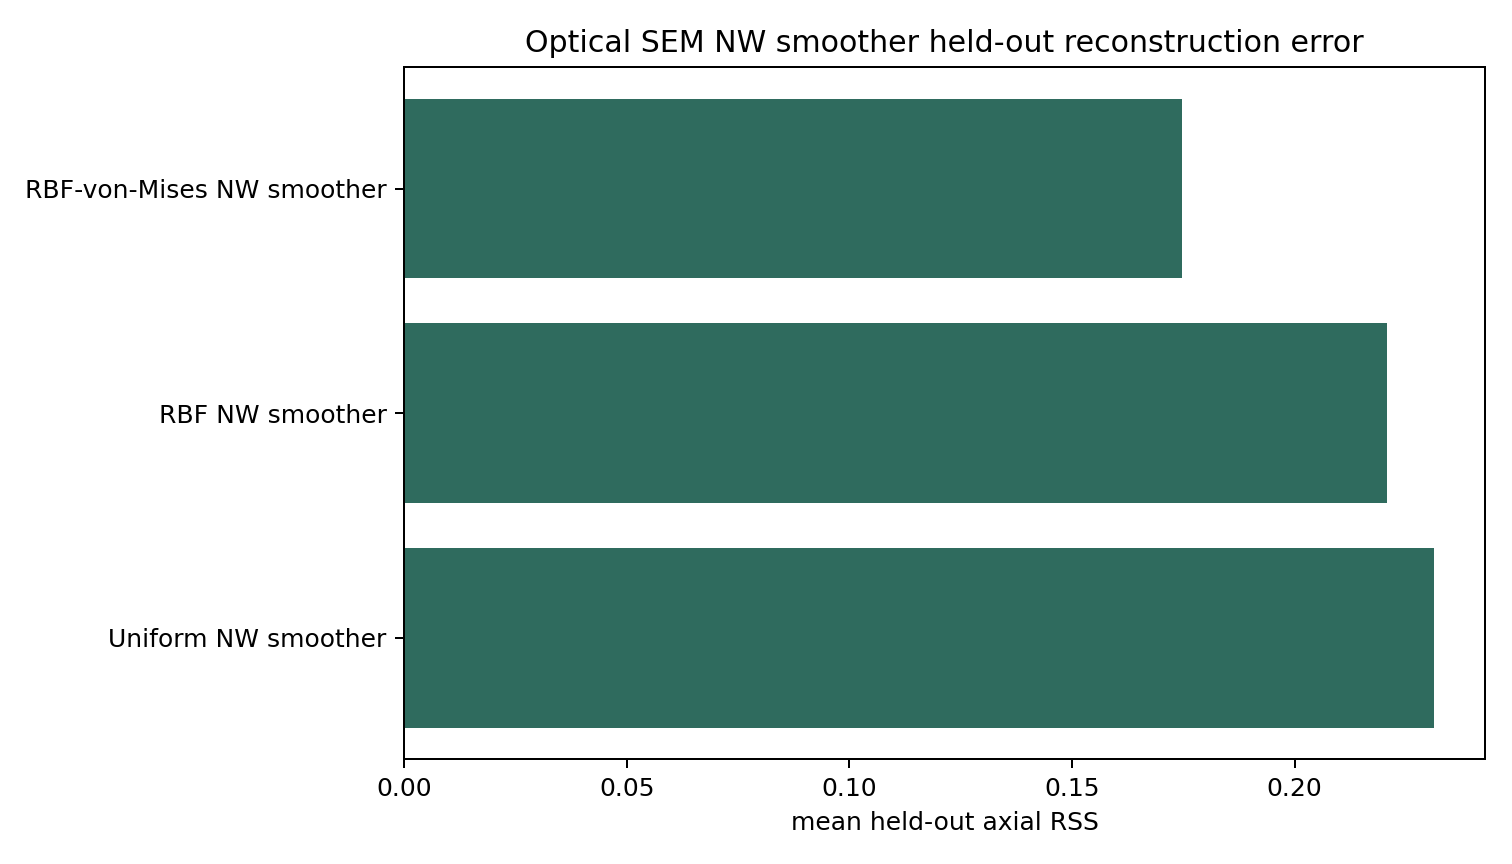
\includegraphics[width=0.78\linewidth]{nw_smoother_mean_rss.png}
\caption{Mean held-out axial RSS for optical SEM local NW smoothers.}
\end{figure}
\begin{figure}[h]
\centering
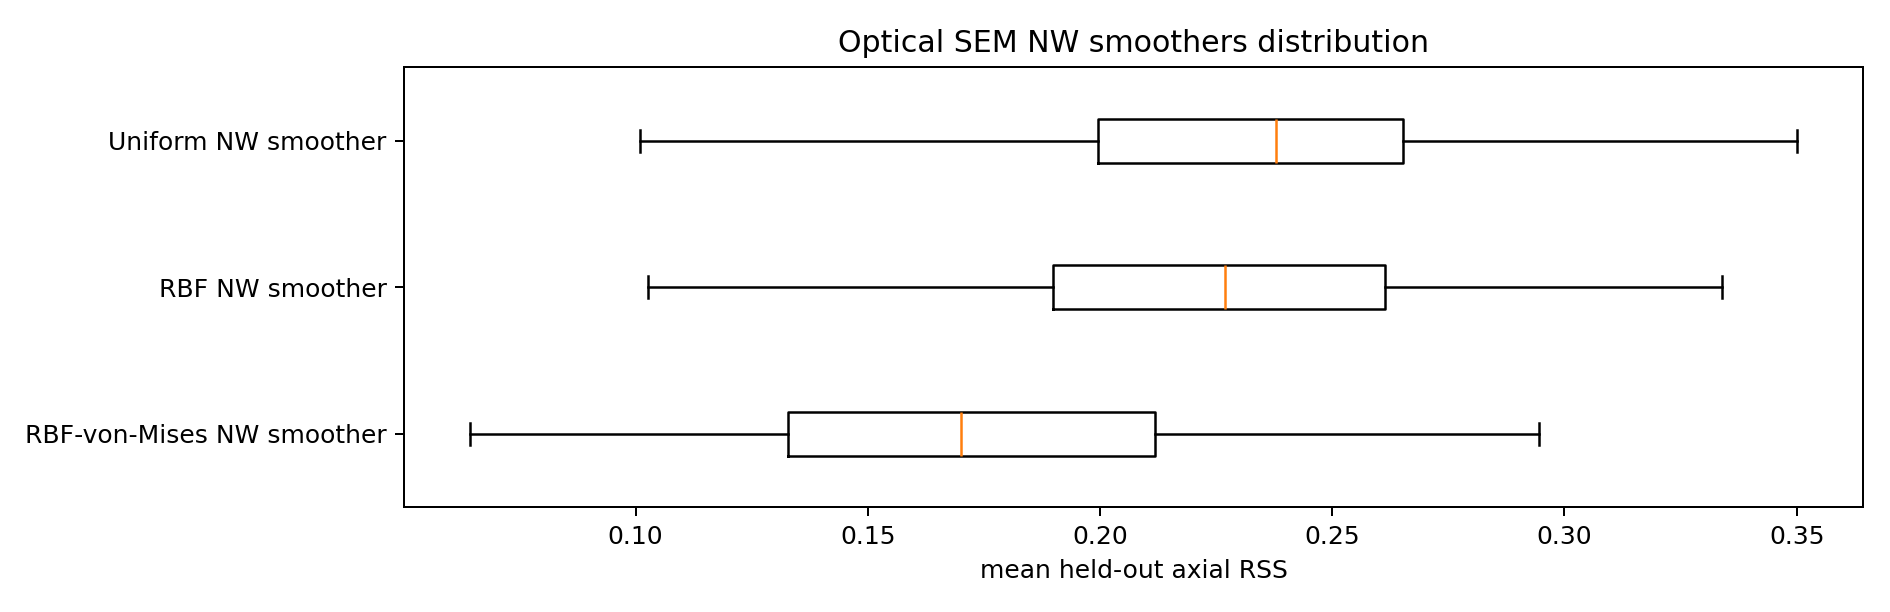
\includegraphics[width=0.86\linewidth]{nw_smoother_boxplot.png}
\caption{Held-out axial RSS distribution for the selected local NW smoothers.}
\end{figure}
\end{document}
